%%%%%%%%%%%%%%%%%%%%%%%%%%%%%%%%%%%%%%%%%
% Template
% LaTeX Template
% Version 1.0 (December 8 2014)
%
% This template has been downloaded from:
% http://www.LaTeXTemplates.com
%
% Original author:
% Brandon Fryslie
% With extensive modifications by:
% Vel (vel@latextemplates.com)
%
% License:
% CC BY-NC-SA 3.0 (http://creativecommons.org/licenses/by-nc-sa/3.0/)
%
% Authors:
% Sabbir Ahmed
% 
%%%%%%%%%%%%%%%%%%%%%%%%%%%%%%%%%%%%%%%%%

\documentclass[paper=usletter, fontsize=12pt]{article}
%%%%%%%%%%%%%%%%%%%%%%%%%%%%%%%%%%%%%%%%%
% Contract Structural Definitions File Version 1.0 (December 8 2014)
%
% Created by: Vel (vel@latextemplates.com)
% 
% This file has been downloaded from: http://www.LaTeXTemplates.com
%
% License: CC BY-NC-SA 3.0 (http://creativecommons.org/licenses/by-nc-sa/3.0/)
%
%%%%%%%%%%%%%%%%%%%%%%%%%%%%%%%%%%%%%%%%%

\usepackage{geometry} % Required to modify the page layout
\usepackage{multicol}
\usepackage{amsmath}
\usepackage{amssymb}

\usepackage[pdftex]{graphicx}
\usepackage{wrapfig}
\usepackage[font=scriptsize, labelfont=bf]{caption}
\usepackage[utf8]{inputenc} % Required for including letters with accents
\usepackage[T1]{fontenc} % Use 8-bit encoding that has 256 glyphs

\usepackage{avant} % Use the Avantgarde font for headings
\usepackage{courier}
\usepackage{xparse}
\usepackage{xcolor}
\usepackage{listings}  % for code verbatim and console outputs

\setlength{\textwidth}{16cm} % Width of the text on the page
\setlength{\textheight}{23cm} % Height of the text on the page
\setlength{\oddsidemargin}{0cm} % Width of the margin - negative to move text left, positive to move it right
\setlength{\topmargin}{-1.25cm} % Reduce the top margin

\setlength{\parindent}{0mm} % Don't indent paragraphs
\setlength{\parskip}{2.5mm} % Whitespace between paragraphs
\renewcommand{\baselinestretch}{1.5}

\definecolor{green}{rgb}{0.18, 0.55, 0.34}

\graphicspath{ {figures/} }
\captionsetup[table]{skip=10pt}

\lstset{language=C, keywordstyle={\bfseries \color{black}}}

% defines algorithm counter for chapter-level
\newcounter{nalg}[section]

%defines appearance of the algorithm counter
\renewcommand{\thenalg}{\thesection .\arabic{nalg}}

% defines a new caption label as Algorithm x.y
\DeclareCaptionLabelFormat{algocaption}{Algorithm \thenalg}

% defines the algorithm listing environment
\lstnewenvironment{pseudocode}[1][] {
    \refstepcounter{nalg}  % increments algorithm number
    \captionsetup{font=normalsize, labelformat=algocaption, labelsep=colon}
    \lstset{
        breaklines=true,
        mathescape=true,
        numbers=left,
        numberstyle=\scriptsize,
        basicstyle=\footnotesize\ttfamily,
        keywordstyle=\color{black}\bfseries,
        keywords={input, output, return, parallel, function, for, to, in, if,
        else, foreach, while, and, or, new, print},
        xleftmargin=.04\textwidth,
        #1
    }
}{}

\renewcommand{\familydefault}{\sfdefault}  % default font for entire document
 % specifies the document layout and style

\begin{document}

    \documentinfo{\textbf{Question:} 10}{\textbf{DATE:} \today}{Sabbir Ahmed}
    \vspace{-0.1in}

    \section{Background}
    Implement the linear feedback shift register shown on \url{https://en.wikipedia.org/wiki/Linear_feedback_shift_register}.

    The core 16-bit register must be implemented with a 16-bit signal. The the shift should be implemented using a concatenation operator to right-shift with the left-most bit loaded from the output of the XOR gates. Verify that linear-feedback shift-register produces all possible states of a 16-bit register excluding the zero state before repeating its sequence.

    To do this, use a Verilog Test Bench to save the output to a file every clock cycle for at least two full cycles of the pattern. Write C/Python/Java code to verify that the pattern repeats identically at least twice and that no number is repeated or missed during one cycle of the pattern. You should submit all code and output files.

    \section{Implementation}
    The maximal linear shift register of 16 bits were computed, with the feedback polynomial $x^{16}+x^{15}+x^{13}+x^{4}+1$ \cite{maxpolynomial} to generate 65535 terms. The test bench allowed at least 2 cycles of shifting to fully complete until termination.

    The module implementation along with its test bench can be found in the `scripts' directory. A sample of the waveform generated is provided:

    \begin{figure}[ht]
        \begin{center}
            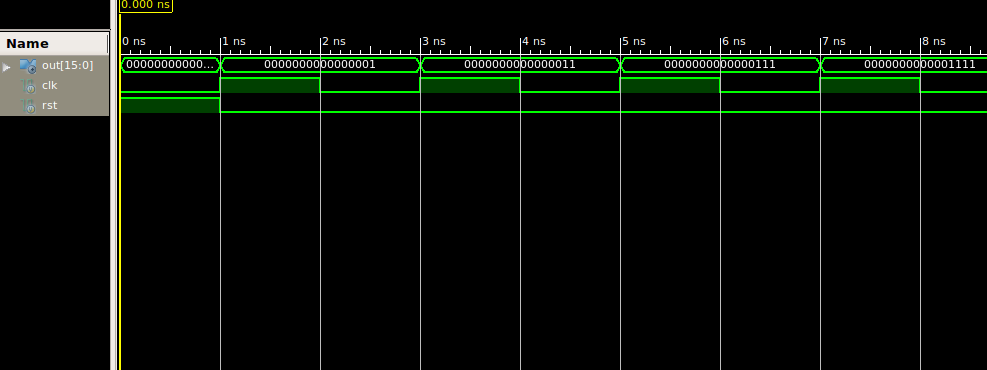
\includegraphics[width=1\textwidth]{wav.png}
            \caption{Waveform Generated from Part 10 Test Bench} \label{fig:wav}
        \end{center}
    \end{figure}

    \section{Testing Validity}
    The terms generated by the linear shift register were dumped to a file for further analysis. A Python script have been provided along with a Makefile for convenience. The Makefile can be used for:
    \begin{itemize}
        \item dumping the outputs to the file with \codeword{make compile}
        \item testing with \codeword{make test}
        \item cleaning up with \codeword{make clean}
        \item handle generation of the LaTex reports
    \end{itemize}

    The Python script reads the output file and iterates through each line to make sure there are no more repetitions of terms than expected. After that, it iterates through the binary representation of all decimal integers from 1 to $2^{16}-1$, and checks if they have been generated in each cycles.

    \begin{figure}[ht]
        \begin{center}
            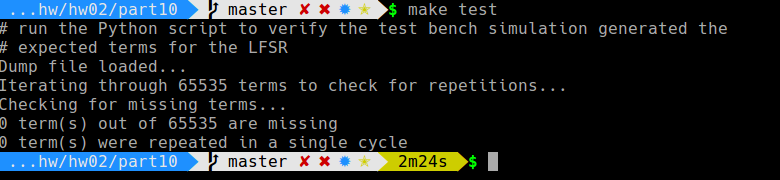
\includegraphics[width=1\textwidth]{testout.png}
            \caption{Output of The Analysis of the Terms Generated by the LSFR} \label{fig:testout}
        \end{center}
    \end{figure}


    \begin{thebibliography}{9}
        \bibitem{maxpolynomial} http://simplefpga.blogspot.com/2013/02/random-number-generator-in-verilog-fpga.html
    \end{thebibliography}

\end{document}
